\begin{sidewaysfigure}[htbp]
\centering 
  \subfloat[\acs{mus} = 0.1, \acs{mur} = 0.4, $v_{inlet}$ = 100 m/s .]
  {
	  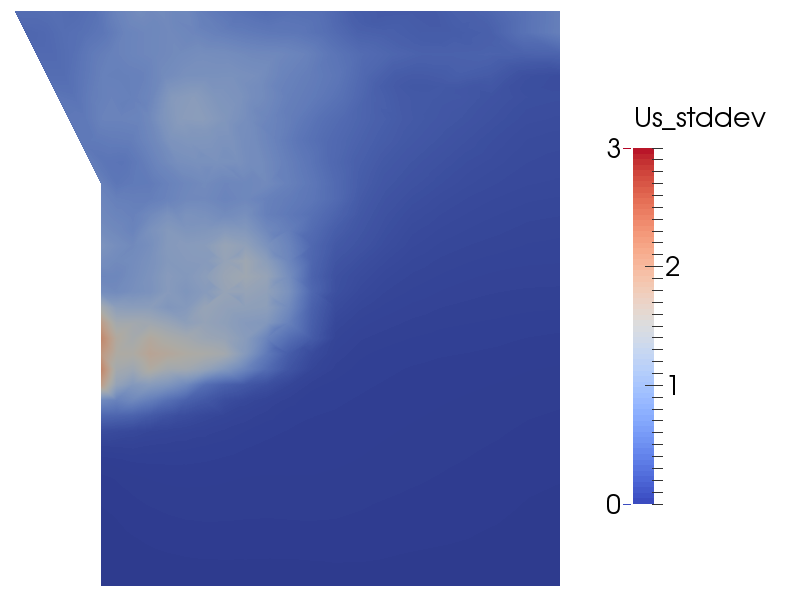
\includegraphics[width=.3\columnwidth]{images/233us_std_lf}
	  \label{fig:233us_std_lf}
  }
  \quad
    \subfloat[\acs{mus} = 0.5, \acs{mur} = 0.4, $v_{inlet}$ = 100 m/s .]
    {
	  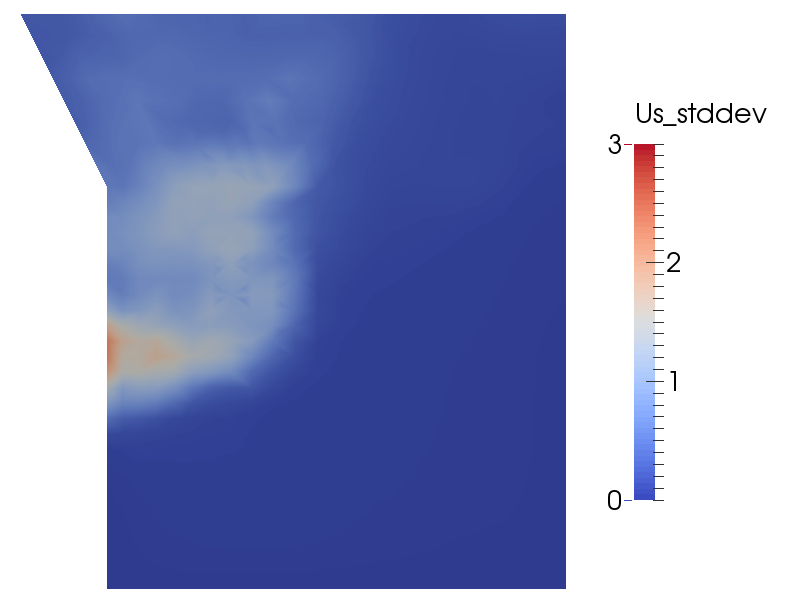
\includegraphics[width=.3\columnwidth]{images/251us_std_mf}
	  \label{fig:251us_std_mf}
  }
  \quad
    \subfloat[\acs{mus} = 0.9, \acs{mur} = 0.4, $v_{inlet}$ = 100 m/s .]
    {
	  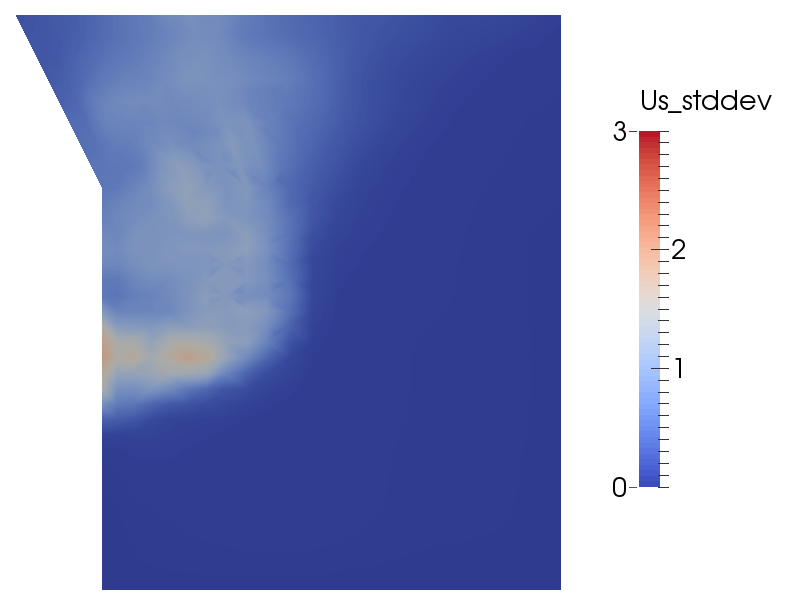
\includegraphics[width=.3\columnwidth]{images/232us_std_hf}
	  \label{fig:232us_std_hf}
  }
  \\
  \subfloat[\acs{mus} = 0.1, \acs{mur} = 0.4, $v_{inlet}$ = 200 m/s .]
  {
	  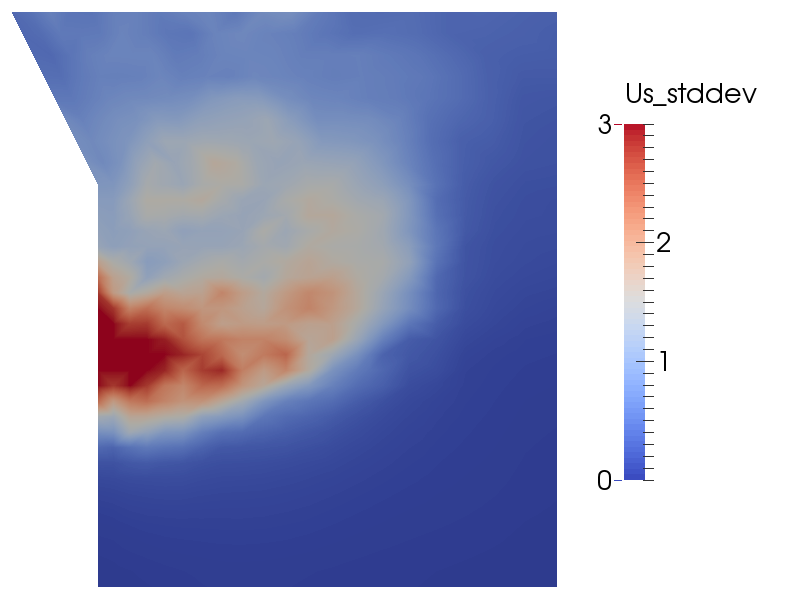
\includegraphics[width=.3\columnwidth]{images/250us_std_lfhv}
	  \label{fig:250us_std_lfhv}
  }
  \quad
    \subfloat[\acs{mus} = 0.9, \acs{mur} = 0.8, $v_{inlet}$ = 100 m/s .]
    {
	  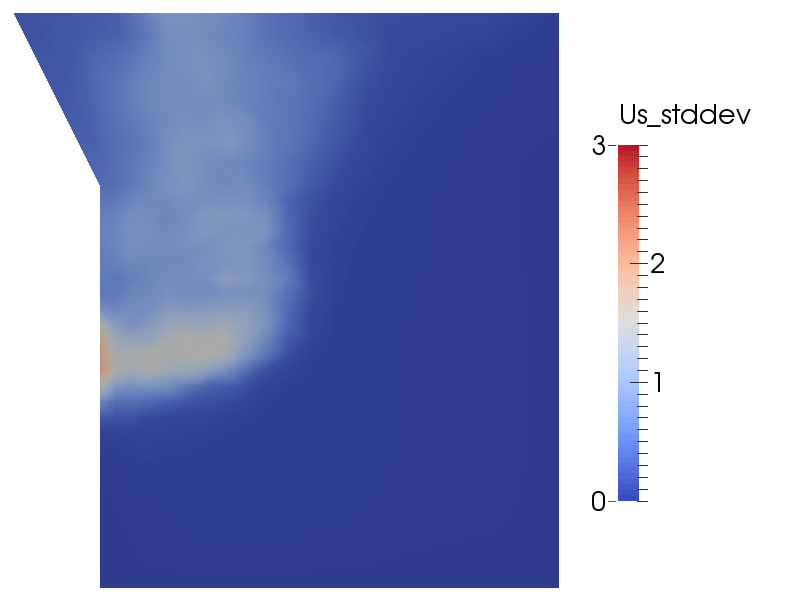
\includegraphics[width=.3\columnwidth]{images/249us_std_hfhr}
	  \label{fig:249us_std_hfhr}  }
  \\
  \caption{Standard deviation particle velocity with different sliding friction
  coefficient.}
  \label{fig:259racewayusstd}
\end{sidewaysfigure}